\chapter{Introduzione}
\label{chap:introduzione}
Nel seguente capitolo viene presetata l'azienda ospitante, il progetto svolto e le motivazioni che hanno 
portato alla scelta di questo argomento per il lavoro di tesi.
\begin{figure}[H]
    \centering
    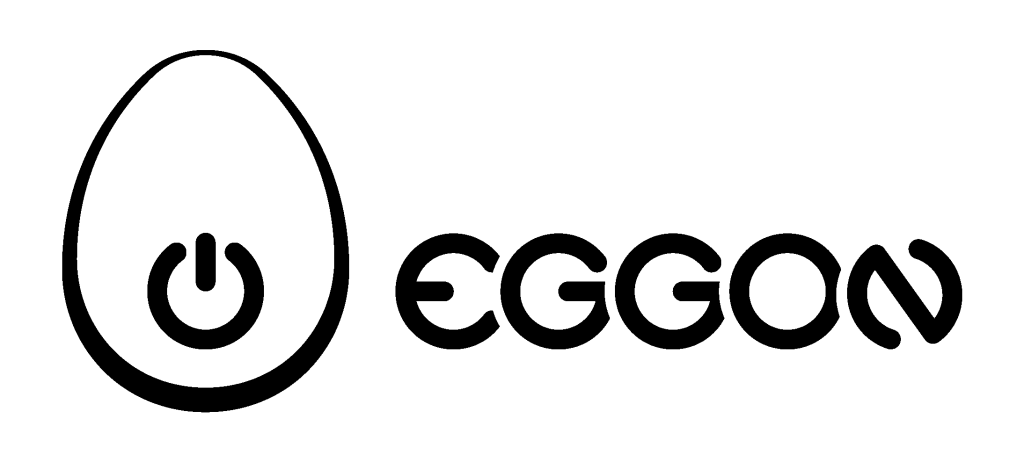
\includegraphics[alt={logo dell'azienda Eggon Srl}, width=.5\columnwidth]{img/logo_eggon.png}
    \caption{Logo di Eggon}
    \label{fig:entanglement}
\end{figure}

Esempio di utilizzo di un termine nel glossario \gls{iiotg}.

Esempio di citazione direttamente nel testo \cite{site:agile-manifesto}.

Esempio di citazione nel piè di pagina \footcite{womak:lean-thinking}.
\section{L'azienda}

Eggon S.r.l. è una software house con sede a Padova che opera in diversi ambiti tecnologici, sviluppando soluzioni software
 innovative e fornendo servizi personalizzati in base alle esigenze dei propri clienti. L’attività dell’azienda si concentra
  principalmente in settori quali la Digital Health, l’Industria 5.0 attraverso lo sviluppo di dispositivi correlati
  all'\gls{iiot} , l’Insurtech e il Fintech, oltre che nell’ambito dell’automazione logistica.

La società nasce dall’esperienza maturata negli Stati Uniti dai suoi fondatori, Gianpaolo Ferrarin e Fulvio Menegozzo, i quali
 hanno successivamente introdotto nel contesto italiano metodologie di lavoro, approcci innovativi e una forte attenzione alla 
 concretezza nello sviluppo di soluzioni tecnologiche.

\section{L'idea}
Introduzione all'idea dello stage\footcite{article:spooky}.
\lipsum[1-3]

\section{Organizzazione del testo}
\begin{description}
    \item[{\hyperref[chap:processi-metodologie]{Il secondo capitolo}}] descrive ...
    
    \item[{\hyperref[chap:descrizione-stage]{Il terzo capitolo}}] approfondisce ...
    
    \item[{\hyperref[chap:analisi-requisiti]{Il quarto capitolo}}] approfondisce ...
    
    \item[{\hyperref[chap:progettazione-codifica]{Il quinto capitolo}}] approfondisce ...
    
    \item[{\hyperref[chap:verifica-validazione]{Il sesto capitolo}}] approfondisce ...
    
    \item[{\hyperref[chap:conclusioni]{Nel settimo capitolo}}] descrive ...
\end{description}

Riguardo la stesura del testo, relativamente al documento sono state adottate le seguenti convenzioni tipografiche:
\begin{itemize}
	\item gli acronimi, le abbreviazioni e i termini ambigui o di uso non comune menzionati vengono definiti nel glossario, situato alla fine del presente documento;
	\item per la prima occorrenza dei termini riportati nel glossario viene utilizzata la seguente nomenclatura: \gls{iiotg};
	\item i termini in lingua straniera o facenti parti del gergo tecnico sono evidenziati con il carattere \textit{corsivo}.
\end{itemize}

\newpage